\documentclass[12pt, dvipdfmx]{beamer}

\renewcommand{\kanjifamilydefault}{\gtdefault}
%%%%%%%%%%%  package  %%%%%%%%%%%
\usepackage{bxdpx-beamer}% dvipdfmxなので必要
\usepackage{pxjahyper}% 日本語で'しおり'したい

\usepackage{amssymb,amsmath,ascmac}

\usepackage{multirow}
\usepackage{bm}

\graphicspath{{../Figures/simulation/}{../Figures/}}

\usepackage{tikz}
\usepackage{xparse}

\usepackage{multimedia}

\usetikzlibrary{shapes,arrows}
%% define fancy arrow. \tikzfancyarrow[<option>]{<text>}. ex: \tikzfancyarrow[fill=red!5]{hoge}
\tikzset{arrowstyle/.style n args={2}{inner ysep=0.1ex, inner xsep=0.5em, minimum height=2em, draw=#2, fill=black!20, font=\sffamily\bfseries, single arrow, single arrow head extend=0.4em, #1,}}
\NewDocumentCommand{\tikzfancyarrow}{O{fill=black!20} O{none}  m}{
\tikz[baseline=-0.5ex]\node [arrowstyle={#1}{#2}] {#3 \mathstrut};}

%微分関連のマクロ
%
\newcommand{\diff}{\mathrm d}
\newcommand{\difd}[2]{\dfrac{\diff #1}{\diff #2}}
\newcommand{\difp}[2]{\dfrac{\partial #1}{\partial #2}}
\newcommand{\difdd}[2]{\dfrac{\diff^2 #1}{\diff #2^2}}
\newcommand{\difpp}[2]{\dfrac{\partial^2 #1}{\partial #2^2}}

%目次スライド
\AtBeginSection[]{
  \frame{\tableofcontents[currentsection]}
}

%アペンディックスのページ番号除去
\newcommand{\backupbegin}{
   \newcounter{framenumberappendix}
   \setcounter{framenumberappendix}{\value{framenumber}}
}
\newcommand{\backupend}{
   \addtocounter{framenumberappendix}{-\value{framenumber}}
   \addtocounter{framenumber}{\value{framenumberappendix}} 
}

\newcommand{\rmd}{\mathrm{d}}
\newcommand{\dd}[1]{\dfrac{\mathrm{d} #1}{\mathrm{d} x}}

%%%
% \usepackage{pgfpages}
% \setbeamertemplate{note page}[plain] % or [default], [compress]
% \setbeameroption{show notes on second screen=right} % or bottom, ...
% \newcommand{\pdfnote}[1]{\note{#1}} % as you like

%%%%%%%%%%%  theme  %%%%%%%%%%%
\usetheme{Copenhagen}
\useoutertheme{default}
%%%%%%%%%%%  font theme  %%%%%%%%%%%
\usefonttheme{professionalfonts}
%%%%%%%%%%%  numbering  %%%%%%%%%%%
% \setbeamertemplate{numbered}
\setbeamertemplate{navigation symbols}{}
\setbeamertemplate{footline}[frame number]

%%%%%%%%%%%%%%%%%%%%%%%%%%%%%%%%%%%
\title
{化学系企業で物理と化学の狭間で\\考えてきたこと}
\subtitle{~コウモリ研究者の戯言~}
\author[東亞合成 佐々木]{佐々木裕}
\institute[東亞合成]{東亞合成}
\date{Nobember 26, 2021}
%%%%%%%%%%%%%%%%%%%%%%%%%%%%%%%%%%
\begin{document}
%%%%%%%%%%%%%%%%%%%%%%%%%%%%%%%%%%
\begin{frame}\frametitle{}
	\titlepage
    \note[item]{こんにちは、東亞合成という会社におります佐々木です。}
    \note[item]{本日はこのようなタイトルでお話をさせていただきます。}
    \note[item]{かなり場違いな話題ですが、まあ、企業の方に何かのお役に立てればと思っております。}
\end{frame}
%%%%%%%%%%%%%%%%%%%%%
\section{はじめに}
%%%%%%%%%%%%%%%%%%%%%%%%%%%%%%%%%%%%%%%%%%%%%
\subsection{はじめに}
\begin{frame}
    \frametitle{はじめに}
    \note[item]{このシンポのタイトルはこのようなものでした。}
    \note[item]{中村先生のオープニングリマークにありましたような、産と官学をつなげるようなきちんとしたお話は、他の方にお任せいたします。クリック}
    \note[item]{で、私のお話はといいますと、私自身に大した実績もあるわけではありませんので、自身の経験を振り返りながら、素人が物事をきちんと理解するためにはどうすればいいんだろうというような立場でお話したいと思います。}
    \note[item]{まあ、単なる与太話ですので、お気楽にお付き合い願えればと。}

    \begin{block}{シンポジウムのタイトル}
        「計算で物事を理解する予測する」\\
        ~産業界の実問題に立ち向かうサイエンス~\\

      22人の計算科学と先端実験の先駆者たちが\\産業界の実問題解決への手掛かりを開示します。
    \end{block}
    \begin{exampleblock}<2>{私のお話}
        \begin{itemize}
            \item 「理解する」という人間の行動について、フォーカス
            \begin{itemize}
                \item 合成化学系出身の企業研究(開発)者が
                \item ソフトマター関連のシミュレーションを通して、
                \item 考えてきたことを紹介。
            \end{itemize}
            \item<2> 21人の計算に関するタイトなお話 + \alert{おまけの与太話}
        \end{itemize}
    \end{exampleblock}
\end{frame}



\subsection{自己紹介}
\begin{frame}
	\frametitle{自己紹介}
    \vspace{-3mm}
    \note[item]{私の背景を理解していただくために、簡単に自己紹介をさせていただきます。}
    \note[item]{教養時代にフラフラしていまして放校になりかけました。}
    \note[item]{そのときに救いの手を差し伸べてくれた先生の関係で、入学当初の思いとは異なる化学系の道へと。}
    \note[item]{就職もうまくいきませんでしたので、仕方なく修士へと進学しました。}
    \note[item]{その時のテーマが、ジビニルエーテルの環化重合によるクラウンエーテル類縁体ポリマーの合成というマニアックなものでした。}
    \note[item]{ちょうど、クラム、ペダーソン、レーンの三人がノーベル賞を取り、ホットな話題となっていました。}
    \note[item]{それでも、アカデミアなんて思いもせずに、お金を稼ぐために民間企業へと。}
        \begin{columns}[T, onlytextwidth]
            \column{.48\linewidth}
                \begin{block}{大学時代}
                    \begin{itemize}
                        \item 大学で三年留年し、\\あわや放校処分
                        \item 望まぬ道の化学系へ\\(合成化学工学科)
                        \item 学部で就職できずに、修士へ
                        \item 研究の面白さに気づく
                        \begin{itemize}
                            \item ジビニルエーテルの環化重合によるクラウンエーテル類縁体
                            \item Host-Guest Chemistry
                        \end{itemize}
                    \end{itemize}
                \end{block}
            \column{.48\linewidth}
                \begin{exampleblock}{企業に就職後}
                    \begin{itemize}
                        \item 合成化学をベースとし、材料設計
                        \begin{itemize}
                            \item ChemDrawの絵を、材料機能へ意味づけ
                            \item 経験知に基づく設計
                        \end{itemize}
                        \item 留学を機会に新規材料
                        \begin{itemize}
                            \item その特性評価から、\\材料設計の道へ
                            \item 例えば、レオロジー
                        \end{itemize}
                        \item その後シミュレーションへ手を広げる
                    \end{itemize}
                \end{exampleblock}
        \end{columns}
\end{frame}

\subsection{モデル化への私のあがき}
\begin{frame}
    \frametitle{私の研究歴}
    \note[item]{ちょっと繰り返しになりますが、もう少し詳しく研究内容を紹介します。}
    \note[item]{メゾスケールシミュレーションへの展開の第一歩は、海外留学時に再発見したオキセタンという4員環環状エーテルでした。}
    \note[item]{オキセタンの特徴的な反応性検討を裏付けるためにミクロなMOシミュレーションの道へ}
    \note[item]{また、高速に固まるだけでは面白さを理解してもらえないので、多様な材料特性を評価するためにレオロジー等の評価技術へと幅を広げていきまして、}
    \note[item]{その流れから、高分子系材料一般の探索指針を求めて、メゾスケールシミュレーションへ。}
    \note[item]{近年は、高分子の振る舞いをきちんと理解していくために、ネットワークポリマーを題材として、破壊靭性についての基礎的な事項を整理しようとしております。}
    \begin{itemize}
        \item もともとは合成ベースの化学系出身
        \item カチオン重合性評価から、MOシミュレーションへ
        \item 高分子系材料一般の探索指針を求めて、メゾスケールシミュレーションへ。
    \end{itemize}
        \begin{block}{実際の内容}
            \begin{itemize}
                \item 光硬化型材料の開発において
                \begin{itemize}
                    \item 各種分子構造の試作と要求特性との相関を模索
                    % \item 光カチオン重合硬化型材料の探索
                    \item オキセタン化合物の有効性の再発見
                \end{itemize}
                \item シミュレーションをベースとしたモデル化へ
                \begin{itemize}
                    \item オキセタンの反応性について
                    \item 表面偏析のモデル化
                    \item ネットワークポリマーとネットワーク理論
                    \item フルアトムMDシミュレーションと粗視化
                \end{itemize}
            \end{itemize}
        \end{block}
\end{frame}

\begin{frame}
    \frametitle{OCTAとの出会い}
        \note[item]{メゾスケールシミュレーションのことの学んだのは、OCTAという統合シミュレータとの出会いがきっかけです。}
        \note[item]{OCTAというのは、当時名古屋大学の土井正雄先生が提唱して、2000年初頭に産官学共同で作り上げたソフトマテリアルに対する統合的なシミュレータです。}
        \note[item]{私自身は、JACIが開催したOCTA-WSに2004年から学ぶ側の素人として参加し、土井先生、川勝先生、滝本先生、および、三菱化学の樹神さんのような多数の民間企業の研究者の知己を得た。}
        \note[item]{OCTAとは、時間、長さのスケールをマルチスケールとして捉え、マルチフィジックスを統合しようとして捉えようとしたアプローチです。}
        \begin{block}{OCTAとは}
            \begin{itemize}
                \item ソフトマテリアルに対する統合的なシミュレータ
                \begin{itemize}
                    \item COGNAC、PASTA、SUSHI、MUFFIN
                    \item GOURMET というシミュレーションプラットフォーム
                \end{itemize}
            \end{itemize}
        \end{block}
        \begin{columns}[c, onlytextwidth]
            \column{.55\linewidth}
            \centering
            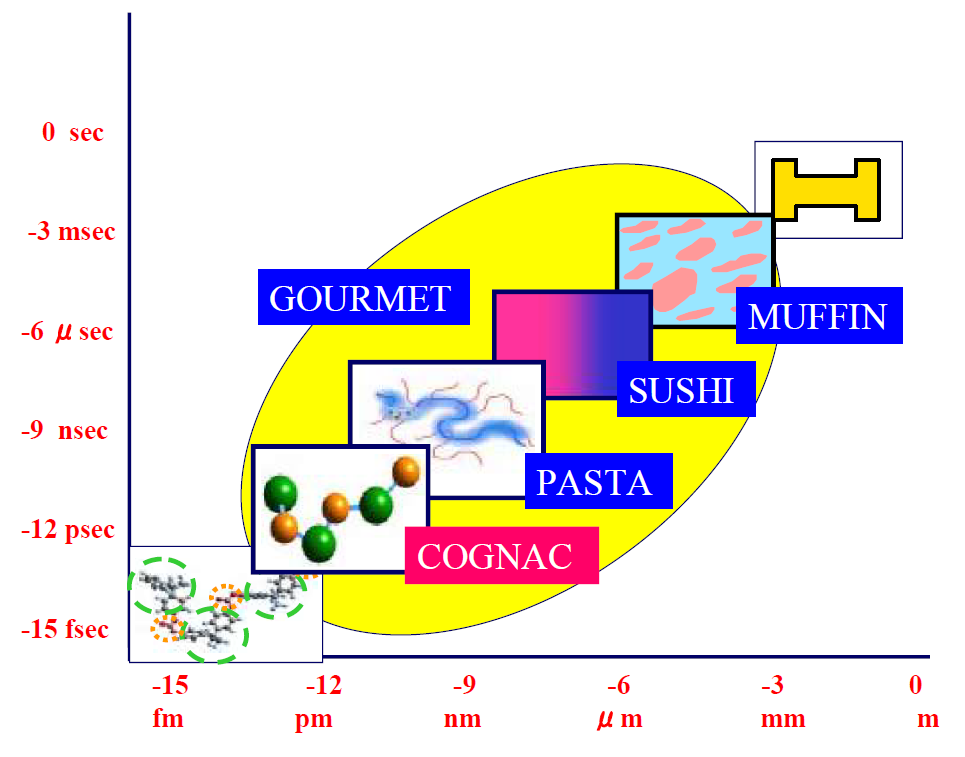
\includegraphics[width=\textwidth]{octa.png}
            \column{.4\linewidth}
                \begin{itemize}
                    \item マルチスケール
                    \item マルチフィジックスの統合
                    \item シームレス\\ズーミング
                \end{itemize}
        \end{columns}    
\end{frame}

\begin{frame}
    \frametitle{統合的な理解を目指して}
    \note[item]{OCAT-WSでの学び、そして議論を通して、やっと、マルチスケールで物事を考えるということを理解し、そして、メゾスケールの重要性に気づいてきました。}
    \note[item]{例えば、ローカルには、熱力学的平衡状態に向けて自由エネルギーを最小化する方向へと遷移するのですが、微視的状態を足し合わせても、グローバルな状態を記述できるとは限りません。}
    \note[item]{また、当然、実事象では平衡状態を達成できるとの担保もないわけです。}
    \note[item]{さらに、開放系での議論も重要になってきます。}
    \note[item]{そんなややこしいものを考えるときに、各スケールで異なる物理があるというマルチフィジックスという取り扱いをしますが、これは、人間の勝手な都合で、}
    \note[item]{実事象の統合的な理解は一筋縄では行かない!}
    \begin{itemize}
        \item マルチスケールな取り扱いで階層的な構造をイメージ
        \begin{itemize}
            \item メゾスケールの重要性
            \begin{itemize}
                \item ローカルには、自由エネルギーを最小化
                \item ローカルの微視的状態の個数倍 $\neq$ グローバル
            \end{itemize}
            \item 実事象では、平衡状態を達成できるとは限らない
            \begin{itemize}
                \item 時間遷移の過程で準安定状態でトラップ
            \end{itemize}
            \item 開放系での議論も重要
            \begin{itemize}
                \item 生物学での、ホメオスタシス(恒常性)
                \item 自己組織化の理解
                % \item 分散システムでの自己安定化:フォールトトレラント
            \end{itemize}
        \end{itemize}
        \item マルチフィジックスは、人間の勝手な都合
        \begin{itemize}
            \item 自然はあるがままに捉えるべき
            \item 階層ごとの切り分けは無意味な場合も多い
        \end{itemize}
        \item シームレスズーミングは幻想
    \end{itemize}
    \large{\alert{実事象の統合的な理解は一筋縄では行かない!}}
\end{frame}

\begin{frame}
    \frametitle{自己組織化という概念}
    \note[item]{例えば、自己組織化という概念を例に考えてみると、工学的には構造ができればいいやという結果オーライな立場で自己集合体とは区別しないことが多くて、ボトムアップ式のナノテクノロジー}
    \note[item]{自己組織化と平衡条件近傍で形成される自己集合体を分離する立場もあるわけです。}
    \begin{block}{自己組織化という概念}
        \begin{itemize}
            \item 材料開発でのナノテクノロジーという文脈で注目
            \item ボトムアップ式のナノテクノロジー
            \item 工学的には、自己集合体とは区別しない事が多い
        \end{itemize}
    \end{block}
    \begin{exampleblock}{自己集合体(平衡条件近傍で形成)とは区別する立場}
        \begin{columns}[T, onlytextwidth]
            \column{.48\linewidth}
            \begin{alertblock}{プリゴジンの散逸構造}
                \begin{itemize}
                    \item 非平衡開放系において
                    \item 平衡構造の不安定化
                    \item 自発的に形成された\\秩序構造
                \end{itemize}
            \end{alertblock}
            \column{.48\linewidth}
            \begin{alertblock}{J.M. Lehn の主張}
                \begin{itemize}
                    \item 超分子科学の提唱者
                    \item 分子自身の分子情報に従って、機能を有する組織を形成
                    % \item 情報の有無に注目
                \end{itemize}
            \end{alertblock}
        \end{columns}
    \end{exampleblock}
\end{frame}

\section{考えてきたこと}
\subsection{モデル化による現象の理解}
\begin{frame}
    \frametitle{モデル化による現象の理解}
    \note[item]{あくまでも、化学系出身の私にとってなんですが、物理系では当たり前の、「自然現象の背後にあるユニバーサリティーの理解と、適正なレベルでのモデル化」という考え方がかけていました。}
    \note[item]{自身の周りを振り返りますと、}
    \begin{alertblock}{化学系の人間としての過去の自身に欠けていたもの}
        物理系では当たり前の考え方\\
        「自然現象の背後にあるユニバーサリティーの理解と、\\適正なレベルでのモデル化」
    \end{alertblock}

    \begin{block}{化学系企業でありがちな状態}
        \begin{itemize}
            \item 教科書的なものの背後にある物理的、数学的な思想を理解することからの逃避
            \item 数式や物理モデルの盲目的な受認によるデータの処理
            \item 統計的な妥当性の確認の放棄
            \item 客観的な視点に基づく独立事象と従属事象の切り分けの放棄
        \end{itemize}
    \end{block}
\end{frame}

\subsection{化学と物理}
\begin{frame}
    \frametitle{化学と物理を比べると}
    \note[item]{化学系の人は、基本的には天下りを受容しがちかと思います。}
    \note[item]{これは有り様を実感できない分子、原子を対象とするため、見えないものを受け入れる}
    \note[item]{一方、これはいいことなんですが、多様性を容認するという雰囲気があります。}
    \note[item]{自由エネルギー、平衡状態、定常状態、等の熱力学の基本が曖昧な場合も多い。}
    \note[item]{ちょっとイチャモンかもしれませんが、偏微分でビビる人が多いのかもしれません}
    \begin{columns}[T, onlytextwidth]
        \column{.5\linewidth}
        \begin{block}{化学のやり方}
            \begin{itemize}
                \item 基本的には天下りを受容
                \begin{itemize}
                    \item 有り様を実感できない分子、原子を対象
                    \item 見えないものを受け入れる
                    \item 「誰が原子を見たか」
                \end{itemize}
                \item 多様性を容認
                \item 熱力学が理解できていない人が、けっこう多い
            \end{itemize}
        \end{block}
        
        \column{.47\linewidth}
        \note[item]{化学系出身の私には、隣の芝生は青いと見えているのかもしれませんが、物理的な考え方は、理論の筋道をきちんと捉えようとしていると感じます。}
        \note[item]{まあ、私がフォーカスしているソフトマター関連の感覚かもしれませんが。} 
        \note[item]{これは、エイヤと私が感心したものを並べただけですが。}
        \begin{exampleblock}{物理的な考え方}
            \begin{itemize}
                \item 事象に内在する一般性
                \item その本質に迫るために\\モデル化
                \item 興味深い考え方:\\
                揺動散逸定理、中心極限定理、線形応答理論、乱雑位相近似、臨界現象(転移における普遍性)、緩和挙動、スケーリング則、無次元化
            \end{itemize}
        \end{exampleblock}
    \end{columns}
\end{frame}

\begin{frame}
    \frametitle{ソフトマターでの印象派物理}
    \note[item]{ソフトマターでは、結構自由な考え方があります。これをほんのタイトルにしたのは御茶ノ水の奥村先生ですが、まあ、以前からあるような流れかと思います。}
    \begin{itemize}
        \item 印象派とは数学的な詳細をあえて大胆に無視することでシンプルに捉え、本質に迫るスタイルのこと
        \item 写実主義的物理との対比
        \item P-G de Gennes からのフランスでの潮流
        \item まわりの実験家とつねに対話をして、身の回りの事象に対して強い好奇心を持ち、斬新なアイデアを創出
        \item 大胆な発想での理解;「大いなる同一視」
    \end{itemize}
\end{frame}

\subsection{抽象的と具体的}
\begin{frame}
    \frametitle{抽象的に考える}
    \note[item]{少し話は変わってきますが、抽象的に考えるということについてです。会社の人の中には、抽象的という言葉に否定的なことも多いかと感じます。}
        \begin{itemize}
            \item 抽象的ということを非現実的と捉え、「えそらごと」と読んでしまう人のなんと多いことか。
        \end{itemize}
    \begin{exampleblock}{抽象とは}
        「抽象」という語については、「事物や表象からある性質・共通性・本質を抽(ひ)き出して把握する」つまり「象を抽き出す」という意味を持つ語
        \begin{itemize}
            \item 個々の事物の本質・共通の属性を抜き出して、\alert{一般的な概念をとらえる}さま。
            \item 単に概念的に思考されるだけで、実際の形態・内容を持たないさま。
        \end{itemize}
        \textcolor{blue}{後者の意味の反意語は、具体的}
    \end{exampleblock}
    \large{\alert{抽象化は、モデル化に必須。}}
\end{frame}

\begin{frame}
    \frametitle{最近の風潮}
            \begin{block}{最近の風潮}
                \begin{itemize}
                    \item 実事象はあまりに複雑で因果関係がわかりにくいにも関わらず、すぐに成果を求める。
                    \item 具体的な対策、方法論を望む。
                    \item シミュレーションに対しても考え方の指針ではなく、\\答えを求める。
                    \item 概念的なものをあまり重視しない。
                    \item そのようなアプローチは、汎用性を生み出さない。
                \end{itemize}
            \end{block}
\end{frame}

\begin{frame}
    \frametitle{単純化して概念へと昇華する方法論}

            \begin{exampleblock}{抽象と捨象}
                \begin{itemize}
                    \item 捨象は捨てる行為に、フォーカスする。
                    \item 単純化する際に、抽き出す行為と捨てる行為
                    \item どちらも不要なものに埋もれた中から、\\本質につながる単純化
                    \item 粗視化はどちらであるべきか?
                    \item 高校時代の美術の熊井先生の走り回り画法
                    \begin{itemize}
                        \item 目を細めて対象物を眺め、ディーテールを無視して、\\目に留まる主要な色を用いて下書き
                        \item 全体に共通なトーンや色合いの部分を、\alert{全体に筆を走り回らせ}ながら書き込む。
                        \item 段階的に、微細なディーテールへと
                    \end{itemize}
                \end{itemize}
            \end{exampleblock}
\end{frame}

\section{私のおすすめ}
\subsection{あるべき状態}
\begin{frame}
    \frametitle{MI への違和感}
    \note[item]{まあ、これは、私の勝手な偏見に基づくものかなとは思っているのですが、MIに対してはかなり違和感を持っております。}
    \note[item]{機械学習に関しては、特定の分野では非常に有効だろうなとは感じております。}
    \note[item]{悪口ばかりでも何なんで、使い方次第とは思います。}
    \note[item]{例えば、ランダムフォレスト等を用いて、説明変数や目的変数の交絡状態を評価したりすること自体は有用かと。}
    \note[item]{でも、やはり、統計モデリングと言われるような手法と、MIとは、なんだか色合いが異なるように感じるのです。}
    \note[item]{これは、嗜好の問題なんでしょうけれど、物理的に意味を持つモデリングを形成することこそが、後の展開を広げられるのではないかと。}
    \note[item]{昨日の実験科学のセッションの発表でも、物理的に意味を持つような説明変数や目的変数をうまく見つけ出して、その因果関係を納得できる道筋でつなげていくことが大事なのかなと感じるのです。}
    \note[item]{この辺の感覚は、先日、講演をお聞きした九大の廣瀬准教授のアプローチには納得するものがあったことはお伝えしておきます。}
    \begin{block}{機械学習について}
        機械学習は特定の分野では非常に有効
        \begin{itemize}
            \item 回帰的手法をベースとした多変量解析
            \item 自動運転のようなフィードバック系
        \end{itemize}
    \end{block}
    \begin{exampleblock}{MI への違和感}
        
        \begin{itemize}
            \item (一部の方に見られる)思考を放棄したような無手勝流
            \item 少なくとも、MI を打ち出の小槌と捉えてはいけない。
            \item シミュレーションを実験の代替とする方法論は有効。
            \item 考えるための道具として有効活用すべき。
            \item 因果推論も確からしくできるようになってきたらしい\\(昨日の杉山先生のお話)
        \end{itemize}
    \end{exampleblock}
\end{frame}

\begin{frame}
    \frametitle{あるべき状態}
    \begin{exampleblock}{化学系研究者の立ち位置}
        \begin{itemize}
            \item 試行錯誤ベースで実際に物質を合成することは必須
            \item 物理側からの理論的な成果を盲目的に受容しては駄目
        \end{itemize}
    \end{exampleblock}
    \begin{alertblock}{あるべき状態}
        \begin{itemize}
            \item 物理的な思考による事象の成り立ちの理解、および、モデル化への道すじを共有
            \item 目的を明確にし、適切な次元、スケール及び時間軸で、議論を行う
            \item 物質の多様性を前提とした化学的な方法論の整理と、適正なモデル化への挑戦
            \item 物理及び化学双方の方法論についての相互理解の深化
        \end{itemize}
    \end{alertblock}
\end{frame}

% \begin{frame}
%     \frametitle{基礎知識の汎用化について}
%         \begin{exampleblock}{データサイエンスの企業での使いこなし}
%             \begin{itemize}
%                 \item データサイエンティストの中途採用
%                 \begin{itemize}
%                     \item マネージメントの難しさ $\Rightarrow$ プロの持ち腐れ
%                     \item 現役データサイエンティストの満足度は低い
%                     \begin{itemize}
%                         \item 手本がない
%                         \item 周りの理解がない
%                         \item スキルアップの時間がない
%                     \end{itemize}
%                 \end{itemize}
%             \end{itemize}
%         \end{exampleblock}
%         \begin{alertblock}{「データサイエンスの民主化」}
%             \begin{itemize}
%                 \item 文系、数学苦手は関係ない
%                 \item データをもとに客観的に考えるという基本的な概念
%                 \item 関係者みんなに広く浅く(深いに越したことはない)
%             \end{itemize}
%         \end{alertblock}
%         \centering
%         \Large{\alert{研究一般についても大事}}
% \end{frame}

\subsection{私のやり方}
\begin{frame}
    \frametitle{私のやり方}
        \begin{itemize}
            \LARGE
            \item 急がば回れ
            \begin{itemize}
                \Large
                \item<2-> 慌ててやっても無駄
                \item<2-> ゆっくりキチンと組み立てる
            \end{itemize}
            \item 備えよ常に
            \begin{itemize}
                \Large
                \item<3-> 見えないものにも前もって
                \item<3-> 泥縄にならないように
            \end{itemize}
            \item 腑に落とす(落ちる)
            \begin{itemize}
                \Large
                \item<4> 消化して使いこなす
                \item<4> 頭でっかちにならない
            \end{itemize}
        \end{itemize}
\end{frame}

% \begin{frame}
%     \frametitle{概念の理解}
%         説明変数と目的変数との関係をモデル化
%         \begin{itemize}
%             \item 例えば、ランダムフォレスト
%             \begin{itemize}
%                 \item 説明変数の選択への制約が少ない。
%                 \item 過学習を影響を排除しやすい。
%             \end{itemize}
%             \item 
            
%         \end{itemize}
% \end{frame}

\subsection{自分の頭で考える}
\begin{frame}
    \frametitle{他人の意見について}
        \begin{columns}[c, onlytextwidth]
            \column{.54\linewidth}
            \large
            \begin{block}{その道のプロの言うこと}
                \begin{itemize}
                    \large
                    \item それなりの確からしさ
                    \item 前提条件の確認が必要
                    \begin{itemize}
                        \large
                        \item 常識が異なる
                        \item 暗黙の了解が多数
                    \end{itemize}
                    \item 素人が下手に使う怖さ
                \end{itemize}
            \end{block}
            \column{.02\linewidth}
            \column{.44\linewidth}<2>
            \LARGE
                \alert{「盲目的に\\信じてはだめ」}
        \end{columns}
\end{frame}

\begin{frame}
    \frametitle{自分の頭で考える}
        \begin{alertblock}{胃の腑に落とすということは?}
            無理やり胃に落としてもだめ!!
        \end{alertblock}
        \begin{columns}[T, onlytextwidth]
            \column{.48\linewidth}
            \vspace{-3mm}
            \begin{block}{咀嚼するための基礎学力}
                STEAM 
                \begin{itemize}
                    \item Science
                    \item Technology
                    \item Engineering
                    \item \alert{Art}
                    \begin{itemize}
                        % \item<2> 体系立てて捉える
                        \item<2-> 成り立ちの美しさ
                        \item<2-> 哲学的な統一性 
                    \end{itemize}
                    \item Mathematics
                \end{itemize}
            \end{block}
            \column{.48\linewidth}
                \centering
                    \includegraphics[width=\textwidth]{steam.png}

                    \footnotesize{https://steam-japan.com/about/}
        \end{columns}
\end{frame}

\begin{frame}
    \frametitle{自分の頭で考える}
        \begin{alertblock}{胃の腑に落とすということは?}
            無理やり胃に落としてもだめ!!
        \end{alertblock}
        \begin{columns}[T, onlytextwidth]
            
            \column{.48\linewidth}  
            \vspace{-3mm}
            \begin{block}{咀嚼するための基礎学力}
                STEAM 
                \begin{itemize}
                    \item Science
                    \item Technology
                    \item Engineering
                    \item \alert{Art}
                    \begin{itemize}
                        % \item<2> 体系立てて捉える
                        \item 成り立ちの美しさ
                        \item 哲学的な統一性 
                    \end{itemize}
                    \item Mathematics
                \end{itemize}
            \end{block}
            
            \column{.48\linewidth}
            \vspace{-3mm}
            \begin{exampleblock}{消化(使いこなす)ために?}
                \begin{itemize}
                    \item 特定分野に囚われない広範な知見
                    \item 締め切りを決めない
                    \item ゆっくり考える
                    \item 自由な議論
                    \item 数値化にこだわらない
                    \item 目に見えないものを\\大事に
                \end{itemize}
            \end{exampleblock}
        \end{columns}
\end{frame}

\begin{frame}
    \frametitle{まとめに代えて}
        \begin{exampleblock}{私のアプローチ}
            \begin{itemize}
                \item 自由に議論できる場の創設
                \begin{itemize}
                    \item Slack を利用して、「東海ソフトマター」を設置
                    \item 大学、企業半々程度の参加者
                    \item それをベースに、Web会議で「ザツダン会」を開催
                \end{itemize}
                \item 基本的な知見の再整理
                \begin{itemize}
                    \item Moodle システムを利用して、LMSサイトを整備中
                    \item 自身の初心者としての疑問点にフォーカスして整理
                    \item 対象:レオロジー、高分子物理、統計等
                \end{itemize}
                \item 定年後のセミナー会社
                \begin{itemize}
                    \item 上記の基礎的な事項に関するセミナー、オンデマンド
                    \item 学生は無料
                \end{itemize}
            \end{itemize}
        \end{exampleblock}
\end{frame}
\end{document}
